% !TEX program = pdflatex
\documentclass[journal]{IEEEtran}

% ============================================================
%  Packages
% ============================================================
\usepackage[T1]{fontenc}
\usepackage{amsmath,amssymb,amsfonts}
\usepackage{algorithmic}
\usepackage{algorithm}
\usepackage{array}
\usepackage{booktabs}
\usepackage{multirow}
\usepackage{cite}
\usepackage{graphicx}
\usepackage{textcomp}
\usepackage{xcolor}
\usepackage{url}
\usepackage{hyperref}
\usepackage{tikz}
\usepackage{tabularx}
\usepackage{threeparttable}
\usepackage{makecell}
\usepackage{enumitem}
\usepackage{balance}
\usepackage{subcaption}

\usetikzlibrary{positioning, arrows.meta, shapes.geometric, fit, backgrounds, calc, decorations.pathreplacing}

\hypersetup{
  colorlinks=true,
  linkcolor=black,
  citecolor=black,
  urlcolor=blue
}

\setlist{nosep}

% Custom commands
\newcommand{\ie}{\textit{i.e.}}
\newcommand{\eg}{\textit{e.g.}}
\newcommand{\etal}{\textit{et al.}}

\begin{document}

% ============================================================
%  Title
% ============================================================
\title{AMTTP: A Four-Layer Architecture for Deterministic Compliance Enforcement in Institutional DeFi}

\author{
  \IEEEauthorblockN{Odeyemi Olusegun Israel}
  \IEEEauthorblockA{Independent Researcher\\
  Derby, United Kingdom\\
  Email: segettii@gmail.com}
}

\maketitle

% ============================================================
%  Abstract
% ============================================================
\begin{abstract}
Decentralised finance has remarkably compressed timeframe, redrawn the contours of global capital markets---automating transactions, dispensing with intermediaries, collapsing settlement cycles. Institutional involvement, for all that still remains strikingly low. The reason is not obscure. No enforceable compliance mechanism operates at the protocol layer; once a transaction achieves on-chain confirmation, it cannot be recalled, reversed, or meaningfully contested. The compliance apparatus that does exist is overwhelmingly retrospective, generating alerts well after settlement rather than preventing illicit transfers outright. Regulated entities carry the exposure. The UK Financial Conduct Authority, through CP25/41, has put the matter beyond doubt: effective pre-settlement controls are now an explicit regulatory expectation~\cite{fca2025}.

We present AMTTP Version~4.0. The system is organised as a four-layer architecture whose express purpose is deterministic compliance enforcement within institutional DeFi environments. Layer~I furnishes SDKs, REST APIs, and web applications for programmatic and human interaction. Layer~II implements a compliance orchestrator---coordinating machine learning risk scoring, graph analytics, sanctions screening, and policy adjudication before consolidating them into a deterministic decision matrix. Layer~III specifies an offline training pipeline: a composite teacher---autoencoder-enhanced XGBoost ($w{=}0.4$), seven FATF AML pattern rules ($w{=}0.3$), and graph-structural properties ($w{=}0.3$)---generates pseudo-labels across 2.64~million transactions for the student pipeline. Layer~IV houses the deployment infrastructure: 13 smart contracts on Ethereum Sepolia, 17 containerised microservices, and a data persistence tier spanning MongoDB, Redis, Memgraph, and IPFS.

Security provisions include multi-oracle threshold signatures, replay protection, and zkNAF---a zero-knowledge proof framework enabling privacy-preserving verification of KYC credentials, risk ranges, and sanctions non-membership. TLS encryption, rate limiting, Cloudflare Tunnel integration, and a UI Integrity Service round out the infrastructure-level safeguards.

The central claim of this paper is that deterministic compliance can be woven directly into DeFi at the architectural level, and the full specification is published as infrastructure-as-code to substantiate that claim.\footnote{Source code: \url{https://github.com/segetii/fintech}}
\end{abstract}

\begin{IEEEkeywords}
DeFi Compliance, AML, Oracle Architecture, Transaction Enforcement, Institutional Finance, Smart Contracts, Zero-Knowledge Proofs
\end{IEEEkeywords}

% ============================================================
%  I. INTRODUCTION
% ============================================================
\section{Introduction}

Decentralised finance has upended much of what was settled about financial infrastructure. Transactions execute on blockchain networks without brokers, clearing houses, or custodians---cutting costs, compressing settlement to seconds, sidelining whole classes of intermediary. The efficiency dividend is real. But so is the compliance deficit, and nowhere more acutely than for institutional actors: pension schemes, sovereign wealth vehicles, asset managers, each tethered to demanding regulatory obligations.

Regulators have taken to calling this the `compliance paradox' of DeFi. In legacy finance, a suspect transfer can be frozen mid-flight, scrutinised, and if warranted reversed before it ever reaches settlement. Permissionless blockchains afford no such luxury. On Ethereum, finality arrives in a matter of seconds. After that, the transaction is immutable---a fait accompli. Monitoring tools, however clever, cannot undo what is already done, and institutions that engage without pre-settlement controls court regulatory sanction, reputational harm, and inadvertent entanglement with illicit capital.

The regulatory trajectory is unmistakable. In the United Kingdom, the Financial Conduct Authority is assembling a comprehensive crypto-asset regime with AML and counter-terrorist financing obligations enforceable from October 2027~\cite{fca2025}. Elsewhere the picture is patchwork: overlapping frameworks, divergent expectations, and capital requirements onerous enough to give most institutional treasurers pause.

What passes for DeFi AML tooling today is, by and large, reactive. Chainalysis and Elliptic furnish off-chain analytics; they flag suspicious patterns and generate alerts. Useful, certainly. But none of these platforms can intercept a high-risk transaction before it settles. Academic work---GraphSAGE being perhaps the most prominent example---has substantially sharpened detection accuracy, yet the outputs remain stranded off-chain, disconnected from any mechanism that might actually block a transfer~\cite{hamilton2017}.

This paper introduces AMTTP---the Anti-Money Laundering Transaction Trust Protocol---an architecture engineered to embed compliance directly within the transactional lifecycle. The design fuses ML-based risk scoring with graph-theoretic analysis and deterministic on-chain enforcement through smart contracts, all arranged across four layers. A zero-knowledge framework, zkNAF, enables privacy-preserving compliance attestation in a manner consonant with GDPR constraints~\cite{groth2016}. The system is not speculative; it is containerised, fully deployable, and backed by an operational dashboard for real-time compliance oversight.

% ============================================================
%  II. RELATED WORK
% ============================================================
\section{Related Work}

Scholarship on DeFi compliance has grown sharply over the past five years, propelled by the ever-widening chasm between legacy AML/CFT frameworks and the realities of decentralised protocols. The early literature treated blockchain risk in broad, sometimes impressionistic strokes. More recent work has narrowed its aperture: privacy-preserving regulation, real-time on-chain enforcement, and the particular constraints facing institutional DeFi participants now command the bulk of attention~\cite{joseph2025}.

Commercial AML platforms---Chainalysis, Elliptic, and their contemporaries---rely on centralised monitoring and retrospective analysis. Graph-based tracing, heuristic pattern matching, alert generation: these are well-established capabilities. What none of them can do is halt a transaction on a permissionless ledger where finality is measured in seconds~\cite{memgraph2024}.

On the academic side, machine learning applied to transaction graphs has meaningfully advanced detection. GraphSAGE and related graph neural network architectures capture wallet-level interaction patterns with impressive discrimination; ROC-AUC figures above 0.90 on standard benchmarks are no longer noteworthy~\cite{hamilton2017}. The persistent shortcoming is the same across all such contributions: they function exclusively off-chain and enforce nothing on the ledger.

Mao \etal\ provide a useful synthesis in their survey of 41 commercial platforms and 28 academic prototypes spanning 2015--2025~\cite{mao2025}. They construct taxonomies across regulatory evolution, verification-layer compliance, and lifecycle phases---preventive, real-time, investigative. Web3 architectures, their analysis suggests, can facilitate transaction graph analysis, real-time scoring, cross-chain tracking, and privacy-preserving verification at a fidelity that centralised systems struggle to match. Yet the gaps they identify are not trivial: cross-chain coverage is fragmentary, DeFi interaction monitoring rudimentary, privacy protocol oversight embryonic, and scalability unresolved. The distance between academic demonstration and production deployment remains considerable.

Privacy-preserving approaches sit at the centre of the tension between compliance imperatives and data protection law. Zero-knowledge proofs---Groth16 circuits especially---allow verification of compliance attributes (a non-sanctioned status, say) without disclosing any underlying personal data~\cite{groth2016}. The fit with GDPR is natural, and the implication for institutional adoption significant. zkAML, for instance, leverages ZK-SNARKs for whitelist-based AML within smart contracts, producing cryptographic assurance of regulatory compliance whilst keeping user data opaque. Verifiable credentials extend the principle further: attestation without revelation~\cite{alego2025}.

Multi-agent architectures mark a shift towards proactive enforcement. Khanvilkar \etal\ propose a decentralised multi-agent system that distributes regulatory rules across agents via formal logic, consensus, and zero-knowledge techniques~\cite{khanvilkar2025}. Smart contracts supply immutable audit trails. Reported accuracy exceeds 98\% at low latency; the design eliminates single points of failure and supports cross-jurisdictional operation---requirements that institutional participants cannot treat as optional.

Layered patterns recur across adjacent domains. Four-layer decompositions---ingestion, ledger, processing, audit---appear in compliance frameworks for distributed systems aiming to guarantee consistency, immutability, and traceability~\cite{gade2025}. Blockchain-enabled models in human resource management and fixed-income tokenisation adopt analogous structures to enforce transparency and encode rules~\cite{madanchian2026}. These designs have inspired deterministic on-chain enforcement, but few integrate comprehensive AML pipelines with graph-temporal analytics end to end.

DeFi-specific work has begun to engage seriously with institutional integration. Mohapatra and Raut examine DeFi protocols for corporate treasury and liquidity management, recognising the efficiency gains whilst stressing the governance imperative~\cite{mohapatra2025}. Olanrewaju tackles DeFi-based asset securitisation, mapping compliance and interoperability obstacles and pointing to oracle networks and KYC-integrated contracts as partial solutions~\cite{olanrewaju2025}.

AMTTP draws on all of this and addresses the most glaring omission: proactive, pre-settlement enforcement. Off-chain analytics---ensemble ML, temporal graph analysis---feed into on-chain deterministic actions within a four-layer architecture. Where existing tools observe and alert, AMTTP normalises heterogeneous signals into real-time compliance decisions: approve, review, escrow, or block. zkNAF provides the privacy-preserving attestation layer that bridges reactive surveillance and the institutional-grade enforcement regulated participants actually need~\cite{fca2025,fatf2023}.

The literature, taken as a whole, demonstrates genuine progress in detection and privacy. What it lacks is a full-stack, production-grade protocol for deterministic AML enforcement purpose-built for institutional DeFi. AMTTP occupies that gap~\cite{sivaraju2024,ogunmola2025,campbell2026}.

% ============================================================
%  III. SYSTEM ARCHITECTURE
% ============================================================
\section{System Architecture}
\label{sec:arch}

The protocol is arranged as four layers, illustrated in Fig.~\ref{fig:architecture}. Each layer owns a distinct domain of responsibility---from user-facing interfaces down to on-chain enforcement---and the separation is deliberate: it yields independent scalability, clean module boundaries, and a system that can evolve without wholesale reimplementation.

% ============================================================
%  Fig. 1 — Architecture Diagram (TikZ)
% ============================================================
\begin{figure*}[!t]
\centering
\resizebox{\textwidth}{!}{%
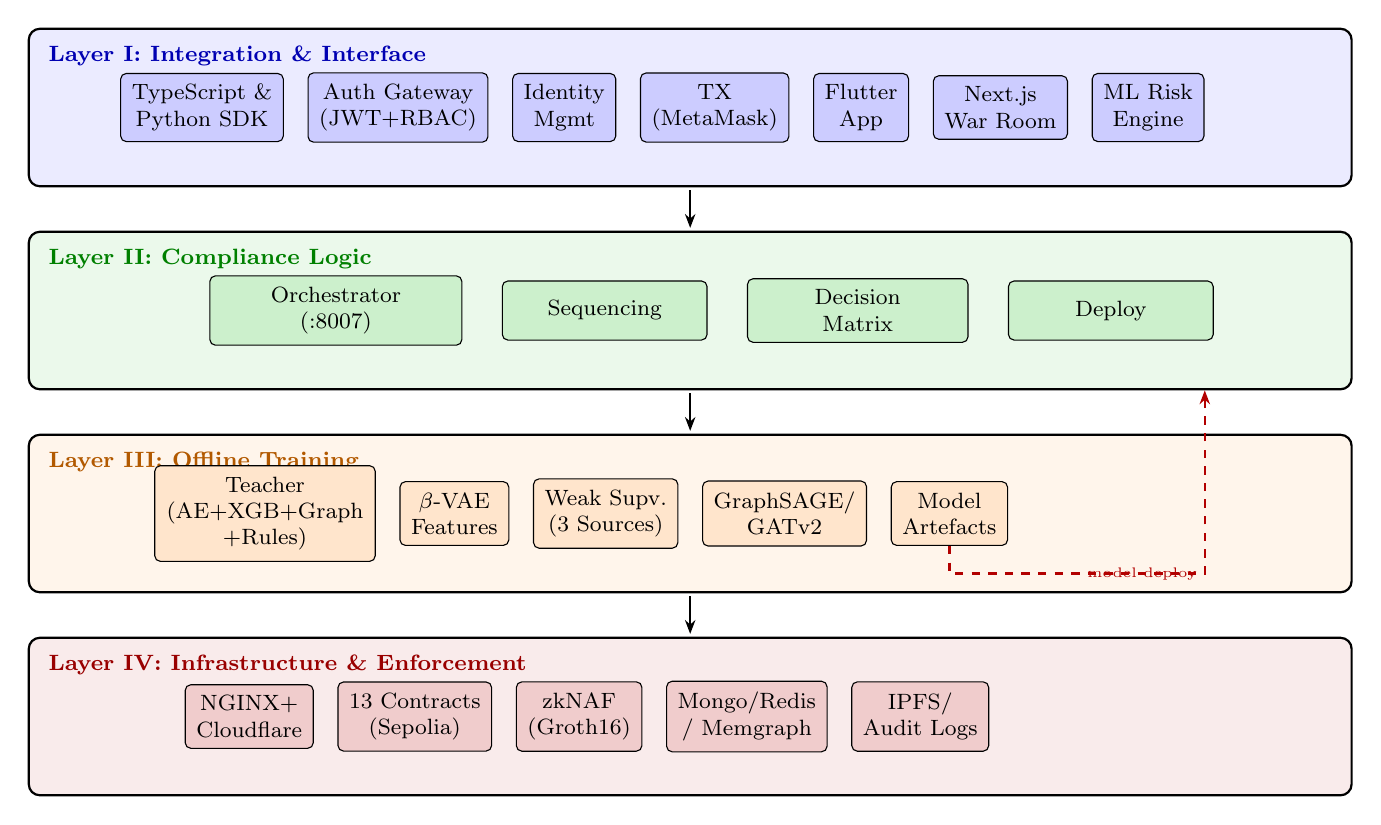
\begin{tikzpicture}[
    node distance=0.35cm and 0.3cm,
    every node/.style={font=\small},
    layer/.style={draw, rounded corners=4pt, minimum width=16.8cm, minimum height=2cm, fill=#1!8, thick},
    block/.style={draw, rounded corners=2pt, minimum height=0.75cm, fill=#1!20, font=\footnotesize, align=center, inner sep=4pt},
    arrow/.style={-{Stealth[length=5pt]}, thick},
    dasharrow/.style={-{Stealth[length=5pt]}, thick, dashed, red!70!black},
    lbl/.style={font=\footnotesize\bfseries, text=#1},
  ]

  % ---- Layer I ----
  \node[layer=blue] (L1) {};
  \node[lbl=blue!70!black, anchor=north west] at ([xshift=4pt, yshift=-3pt]L1.north west) {Layer I: Integration \& Interface};

  % Place blocks symmetrically inside L1
  \node[block=blue] (sdk) at ([xshift=-6.2cm]L1.center) {TypeScript \&\\Python SDK};
  \node[block=blue, right=0.3cm of sdk] (auth) {Auth Gateway\\(JWT+RBAC)};
  \node[block=blue, right=0.3cm of auth] (identity) {Identity\\Mgmt};
  \node[block=blue, right=0.3cm of identity] (tx) {TX\\(MetaMask)};
  \node[block=blue, right=0.3cm of tx] (flutter) {Flutter\\App};
  \node[block=blue, right=0.3cm of flutter] (nextjs) {Next.js\\War Room};
  \node[block=blue, right=0.3cm of nextjs] (mlrisk) {ML Risk\\Engine};

  % ---- Layer II ----
  \node[layer=green!70!black, below=0.55cm of L1] (L2) {};
  \node[lbl=green!50!black, anchor=north west] at ([xshift=4pt, yshift=-3pt]L2.north west) {Layer II: Compliance Logic};

  \node[block=green!70!black, minimum width=3.2cm] (orch) at ([xshift=-4.5cm]L2.center) {Orchestrator\\(:8007)};
  \node[block=green!70!black, minimum width=2.6cm, right=0.5cm of orch] (seq) {Sequencing};
  \node[block=green!70!black, minimum width=2.8cm, right=0.5cm of seq] (matrix) {Decision\\Matrix};
  \node[block=green!70!black, minimum width=2.6cm, right=0.5cm of matrix] (deploy) {Deploy};

  % ---- Layer III ----
  \node[layer=orange, below=0.55cm of L2] (L3) {};
  \node[lbl=orange!70!black, anchor=north west] at ([xshift=4pt, yshift=-3pt]L3.north west) {Layer III: Offline Training};

  \node[block=orange, minimum width=2.8cm] (teacher) at ([xshift=-5.4cm]L3.center) {Teacher\\(AE+XGB+Graph\\+Rules)};
  \node[block=orange, right=0.3cm of teacher] (bvae) {$\beta$-VAE\\Features};
  \node[block=orange, right=0.3cm of bvae] (weaksup) {Weak Supv.\\(3 Sources)};
  \node[block=orange, right=0.3cm of weaksup] (gnn) {GraphSAGE/\\GATv2};
  \node[block=orange, right=0.3cm of gnn] (artefacts) {Model\\Artefacts};

  % ---- Layer IV ----
  \node[layer=red!70!black, below=0.55cm of L3] (L4) {};
  \node[lbl=red!60!black, anchor=north west] at ([xshift=4pt, yshift=-3pt]L4.north west) {Layer IV: Infrastructure \& Enforcement};

  \node[block=red!70!black] (nginx) at ([xshift=-5.6cm]L4.center) {NGINX+\\Cloudflare};
  \node[block=red!70!black, right=0.3cm of nginx] (contracts) {13 Contracts\\(Sepolia)};
  \node[block=red!70!black, right=0.3cm of contracts] (zknaf) {zkNAF\\(Groth16)};
  \node[block=red!70!black, right=0.3cm of zknaf] (data) {Mongo/Redis\\/ Memgraph};
  \node[block=red!70!black, right=0.3cm of data] (ipfs) {IPFS/\\Audit Logs};

  % ---- Arrows between layers ----
  \draw[arrow] ([yshift=-1pt]L1.south) -- ([yshift=1pt]L2.north);
  \draw[arrow] ([yshift=-1pt]L2.south) -- ([yshift=1pt]L3.north);
  \draw[arrow] ([yshift=-1pt]L3.south) -- ([yshift=1pt]L4.north);

  % ---- Dashed arrow: model artefact deployment ----
  \draw[dasharrow] (artefacts.south) -- ++(0,-0.35)
    -| ([xshift=3cm]matrix.east |- L2.south)
    node[pos=0.25, right, font=\tiny, text=red!70!black] {model deploy};

\end{tikzpicture}%
}% end resizebox
\caption{AMTTP four-layer architecture. Layer~I exposes integration interfaces; Layer~II implements compliance decision logic; Layer~III trains models offline via weak supervision; Layer~IV provides infrastructure and on-chain enforcement. The dashed arrow indicates model artefact deployment from the training pipeline to the production risk engine.}
\label{fig:architecture}
\end{figure*}

\subsection{Layer~I: Integration and Interface Layer}

Layer~I is the protocol's public surface. It exposes interfaces for human operators, third-party applications, and automated systems alike.

\textbf{AMTTP Open-Source SDK.} TypeScript and Python client libraries handle transaction construction and signing, maintain WebSocket connections for real-time event streaming, and provide batch scoring interfaces where throughput demands it.

\textbf{RESTful API Interface.} A FastAPI service on port~8000 exposes the production compliance endpoints. \texttt{/score} evaluates individual transactions, returning a risk score alongside explanatory metadata. \texttt{/batch} processes arrays of transactions in a single call. \texttt{/model/info} surfaces model version and feature metadata. \texttt{/alerts} feeds SIEM dashboards; \texttt{/health} serves readiness probes.

\textbf{Web Application Layer.} Two web applications serve distinct audiences. A Flutter-based consumer application plugs into MetaMask, letting end-users connect wallets and inspect risk assessments before signing anything. A separate Next.js `War Room' dashboard gives compliance analysts real-time alert visibility, case management workflows, score visualisations, and a zkNAF proof verification panel.

\subsection{Layer~II: Compliance Logic Layer}

This is where decisions are made. Layer~II ingests transaction data from Layer~I, evaluates risk across several parallel services, and resolves them into a deterministic compliance verdict.

\textbf{Compliance Orchestrator.} The Orchestrator (port~8007) is the coordination hub. When a transaction arrives, it dispatches parallel requests to the ML Risk Engine, the Graph API, the Sanctions service, and the Geo-risk service. Responses are aggregated, enriched with entity profile data, and distilled into a unified risk assessment.

\textbf{Identity Management Module.} Entity profiles---KYC status, historical transaction patterns, jurisdictional metadata---are maintained here, and deterministic rules are applied against each incoming transaction.

\textbf{Transaction Sequencing Module.} Context enrichment is the function of this module: sanctions matches, KYC status, rule-based alerts, geographic risk, fraud probabilities, and confidence levels from the ML model are all appended to the transaction record before decision.

% ============================================================
%  Table I — Compliance Decision Matrix
% ============================================================
\begin{table}[!t]
\centering
\caption{Compliance Decision Matrix}
\label{tab:decision_matrix}
\begin{tabular}{p{5.2cm}l}
\toprule
\textbf{Condition} & \textbf{Action} \\
\midrule
$\text{risk} < 200 \;\wedge\; \neg\text{sanctioned} \;\wedge\; \text{geo} \notin \{\text{PROHIBITED}\}$ & APPROVE \\
$200 \le \text{risk} < 400 \;\wedge\; \neg\text{sanctioned}$ & APPROVE \\
$400 \le \text{risk} < 600 \;\wedge\; \neg\text{sanctioned}$ & REVIEW \\
$600 \le \text{risk} < 800$ & ESCROW \\
$\text{risk} \ge 800 \;\wedge\; \text{red flags}$ & BLOCK \\
$\text{sanctioned} \;\vee\; \text{FATF blacklist}$ & BLOCK \\
$\text{velocity anomaly} \;\wedge\; \text{risk} \ge 400$ & ESCROW \\
$\text{risk} > 600 \;\wedge\; \neg\text{KYC}$ & BLOCK \\
\bottomrule
\end{tabular}
\end{table}

\textbf{ML Risk Engine (Production CPU).} The production engine runs on CPU infrastructure, loading model artefacts from a Docker volume. It evaluates the trained ensemble---XGBoost and LightGBM, combined through a logistic regression meta-learner---against each incoming transaction.

\textbf{Compliance Decision Matrix.} All signals converge on the deterministic action matrix in Table~\ref{tab:decision_matrix}.

\subsection{Layer~III: Offline Training Pipeline}

Layer~III sits entirely offline. Its sole purpose is the development and validation of the machine learning models that the production risk engine consumes. Training runs on GPU infrastructure (Google Colab) and follows a multi-stage weak supervision methodology.

% ============================================================
%  Fig. 2 — ML Pipeline Diagram (TikZ)
% ============================================================
\begin{figure*}[!t]
\centering
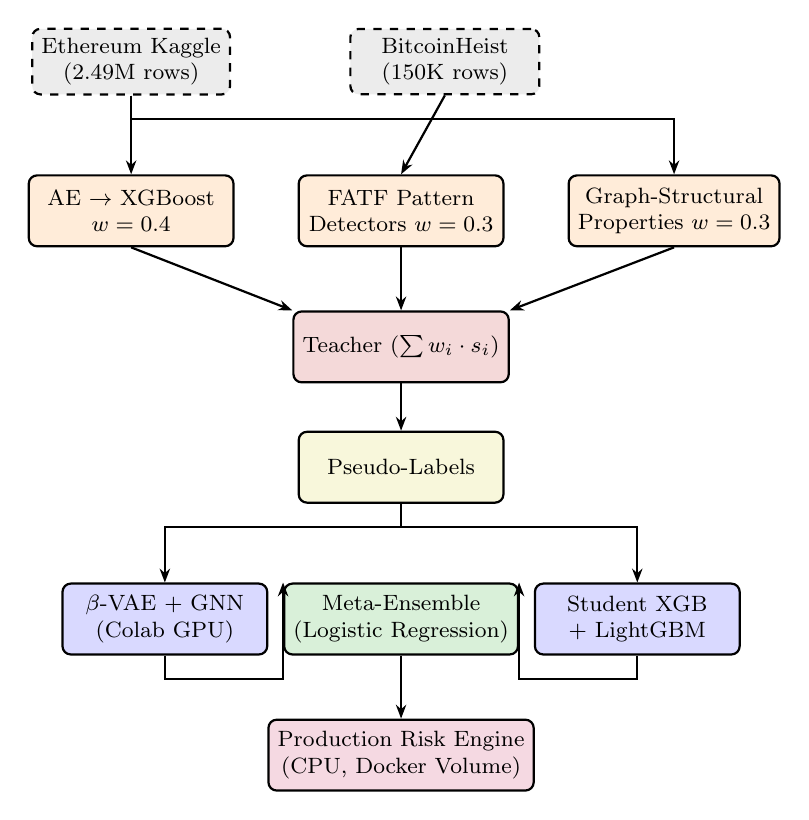
\begin{tikzpicture}[
    node distance=0.5cm and 0.6cm,
    every node/.style={font=\small},
    block/.style={draw, rounded corners=3pt, minimum height=0.9cm, minimum width=2.6cm, fill=#1!15, font=\footnotesize, align=center, thick},
    data/.style={draw, rounded corners=3pt, minimum height=0.8cm, minimum width=2.4cm, fill=gray!15, font=\footnotesize, align=center, thick, dashed},
    arrow/.style={-{Stealth[length=5pt]}, thick},
    weight/.style={font=\tiny, text=red!70!black},
  ]

  % --- Data Sources ---
  \node[data] (eth) {Ethereum Kaggle\\(2.49M rows)};
  \node[data, right=1.5cm of eth] (btc) {BitcoinHeist\\(150K rows)};

  % --- Teacher Components ---
  \node[block=orange, below=1cm of eth] (aexgb) {AE $\to$ XGBoost\\$w = 0.4$};
  \node[block=orange, right=0.8cm of aexgb] (fatf) {FATF Pattern\\Detectors $w = 0.3$};
  \node[block=orange, right=0.8cm of fatf] (graph) {Graph-Structural\\Properties $w = 0.3$};

  % --- Teacher Fusion ---
  \node[block=red!70!black, below=0.8cm of fatf] (teacher) {Teacher ($\sum w_i \cdot s_i$)};
  \node[block=yellow!80!black, below=0.6cm of teacher] (pseudo) {Pseudo-Labels};

  % --- Student Pipeline ---
  \node[block=blue, below=1cm of pseudo, xshift=-3cm] (bvae) {$\beta$-VAE + GNN\\(Colab GPU)};
  \node[block=blue, below=1cm of pseudo, xshift=3cm] (student) {Student XGB\\+ LightGBM};

  % --- Meta-Ensemble ---
  \node[block=green!60!black, below=1cm of pseudo] (meta) {Meta-Ensemble\\(Logistic Regression)};

  % --- Production ---
  \node[block=purple, below=0.8cm of meta] (prod) {Production Risk Engine\\(CPU, Docker Volume)};

  % --- Arrows ---
  \draw[arrow] (eth.south) -- (aexgb.north);
  \draw[arrow] (btc.south) -- (fatf.north);
  \draw[arrow] (eth.south) -- ++(0,-0.3) -| (graph.north);

  \draw[arrow] (aexgb.south) -- (teacher.north west);
  \draw[arrow] (fatf.south) -- (teacher.north);
  \draw[arrow] (graph.south) -- (teacher.north east);

  \draw[arrow] (teacher.south) -- (pseudo.north);

  \draw[arrow] (pseudo.south) -- ++(0,-0.3) -| (bvae.north);
  \draw[arrow] (pseudo.south) -- ++(0,-0.3) -| (student.north);

  \draw[arrow] (bvae.south) -- ++(0,-0.3) -| (meta.north west);
  \draw[arrow] (student.south) -- ++(0,-0.3) -| (meta.north east);

  \draw[arrow] (meta.south) -- (prod.north);

\end{tikzpicture}
\caption{Layer~III offline training pipeline. Two public datasets feed the composite teacher: autoencoder-enhanced XGBoost predictions ($w{=}0.4$), FATF-typology pattern detectors ($w{=}0.3$), and graph-structural properties ($w{=}0.3$) are fused into pseudo-labels. The student pipeline---$\beta$-VAE/GNN and gradient-boosted classifiers---trains on these labels, unified by a logistic regression meta-learner and deployed to the production risk engine.}
\label{fig:ml_pipeline}
\end{figure*}

\textbf{Stage~1---Teacher Model (Hope Machine).} Training data come from two public sources: the BitcoinHeist and Ethereum Kaggle datasets. Together they comprise 2,640,911 rows spanning 177 features, with fraud prevalence at 0.87\%---a 113:1 class imbalance that is, if anything, conservative relative to real-world ratios.

\textbf{VAE Featurisation.} A VAEWithAttention model runs on the GPU, generating latent vectors that compress the original feature space whilst retaining the information that matters. Reconstruction error doubles as an anomaly signal and is appended directly to the feature set.

\textbf{Stage~2---Teacher Labelling.} The teacher is a composite of three weighted signals fused into a single pseudo-label:
\begin{itemize}
  \item \textbf{AE-enhanced XGBoost} ($w = 0.4$): predictions on 1,670 fresh BigQuery transactions, drawing on 171 engineered features augmented with autoencoder latent representations.
  \item \textbf{FATF Pattern Detectors} ($w = 0.3$): seven behavioural rules grounded in AML typologies---SMURFING, FAN\_OUT, FAN\_IN, LAYERING, STRUCTURING, VELOCITY, PEELING.
  \item \textbf{Graph-Structural Properties} ($w = 0.3$): degree centrality, community detection, proximity to known illicit clusters.
\end{itemize}
The weighted combination produces the pseudo-labels on which the student pipeline trains.

\textbf{Stage~3a---Student VAE/GNN Pipeline.} A combined Variational Autoencoder and Graph Neural Network trains on the teacher's pseudo-labels, again using Colab GPU infrastructure.

\textbf{Stage~3b---Production Models (CPU Deployed).} The resulting model artefacts are mounted via Docker volume into the Layer~II risk engine.

\subsection{Layer~IV: Infrastructure and Enforcement Layer}

Layer~IV is the foundation. It bridges off-chain compliance verdicts to deterministic on-chain enforcement.

\textbf{API Gateway.} An NGINX reverse proxy handles TLS termination, rate limiting at 100 requests per second, and path-based routing. Cloudflare Tunnel provides the secure external ingress.

\textbf{On-Chain Verification---Ethereum Smart Contracts.} Thirteen Solidity smart contracts are deployed on Ethereum Sepolia, enumerated in Table~\ref{tab:contracts}.

% ============================================================
%  Table II — Smart Contract Components
% ============================================================
\begin{table}[!t]
\centering
\caption{AMTTP Smart Contract Components}
\label{tab:contracts}
\begin{tabular}{ll}
\toprule
\textbf{Contract} & \textbf{Purpose} \\
\midrule
AMTTPCore & Risk oracle, escrow, threshold sigs \\
AMTTPNFT & KYC badges (ERC-721) \\
DisputeResolver & Kleros arbitration integration \\
CrossChain & LayerZero cross-chain relay \\
PolicyEngine & Rule \& threshold configuration \\
RiskRouter & Multi-chain score routing \\
zkNAFVerifier & Groth16 proof verification \\
SafeModule & Gnosis Safe multi-sig \\
CoreSecure & Hardened variant, reentrancy guards \\
Streamlined & Gas-optimised compliance \\
BiconomyModule & Gasless meta-transactions \\
PolicyManager & Policy \& threshold management \\
\bottomrule
\end{tabular}
\end{table}

% ============================================================
%  Table III — zkNAF Proof Types
% ============================================================
\begin{table}[!t]
\centering
\caption{zkNAF Proof Types}
\label{tab:zknaf}
\begin{tabular}{p{2.6cm}p{4.8cm}}
\toprule
\textbf{Proof Type} & \textbf{Purpose} \\
\midrule
KYC Credential & Verify identity status without revealing personal data \\
Risk Range & Prove risk score within acceptable bounds without disclosing exact value \\
Sanctions Non-Membership & Confirm address is not on watchlists without exposing the full list \\
\bottomrule
\end{tabular}
\end{table}

\textbf{zkNAF Circuits.} Three proof types enable privacy-preserving compliance verification: KYC credential proofs, risk range proofs, and sanctions non-membership proofs (Table~\ref{tab:zknaf}).

\textbf{Data Persistence Layer.} Five storage technologies serve distinct requirements:
\begin{itemize}
  \item \textbf{MongoDB}---entity profiles, alerts, transaction histories, audit trails.
  \item \textbf{Redis}---in-memory caching for sessions, rate limits, sender feature vectors.
  \item \textbf{Memgraph}---the graph layer: entity relationships and risk propagation paths.
  \item \textbf{Helia/IPFS}---immutable audit logs, evidence packages, cryptographic proofs.
  \item \textbf{BigQuery}---training data ingestion: 30 days of Ethereum transactions, approximately 1.67~million records.
\end{itemize}

% ============================================================
%  IV. PRODUCTION IMPLEMENTATION
% ============================================================
\section{Production Implementation}
\label{sec:prod}

The entire system ships as a containerised deployment orchestrated through Docker Compose. Table~\ref{tab:services} catalogues the 24 services, their ports, and their principal functions.

% ============================================================
%  Table IV — Service Infrastructure
% ============================================================
\begin{table*}[!t]
\centering
\caption{AMTTP Service Infrastructure}
\label{tab:services}
\begin{tabular}{llll}
\toprule
\textbf{Service} & \textbf{Port} & \textbf{Purpose} & \textbf{Tech} \\
\midrule
\multicolumn{4}{l}{\textit{Application Services}} \\
NGINX Gateway   & 8888  & Reverse proxy, TLS          & NGINX \\
Flutter App      & 3010  & End-user interface           & Flutter \\
Next.js War Room & 3006  & Compliance dashboard         & Next.js \\
Orchestrator     & 8007  & Decision coord.              & FastAPI \\
ML Risk Engine   & 8000  & Risk scoring                 & FastAPI \\
Graph API        & 8001  & Memgraph interface           & FastAPI \\
FCA Compliance   & 8002  & SAR, Travel Rule, FCA reports & FastAPI \\
Policy Service   & 8003  & Policy CRUD, whitelist/blacklist & FastAPI \\
Sanctions Svc    & 8004  & Watchlist screening          & FastAPI \\
Monitoring Svc   & 8005  & AML rules, alert management  & FastAPI \\
Geo-Risk Svc     & 8006  & Geographic risk              & FastAPI \\
Integrity Svc    & 8008  & UI tamper detection           & FastAPI \\
Explainability   & 8009  & ML XAI, typology analysis    & FastAPI \\
zkNAF Demo       & 8010  & Zero-knowledge proofs        & FastAPI \\
Oracle Service   & 3001  & KYC, PEP, EDD, bulk scoring  & Node.js \\
Auth Gateway     & 8020  & JWT authentication           & FastAPI \\
\midrule
\multicolumn{4}{l}{\textit{Infrastructure Services}} \\
MongoDB          & 27017 & Document store               & MongoDB \\
Redis            & 6379  & In-memory cache              & Redis \\
Memgraph         & 7687  & Graph database               & Memgraph \\
Memgraph Lab     & 3000  & Graph visualisation           & Memgraph \\
Helia/IPFS       & 5001  & Immutable storage            & Helia \\
MinIO            & 9000  & S3-compatible object store   & MinIO \\
HashiCorp Vault  & 8200  & Secrets management           & Vault \\
Hardhat Node     & 8545  & Ethereum dev node            & Hardhat \\
\bottomrule
\end{tabular}
\end{table*}

% ============================================================
%  V. SECURITY MODEL
% ============================================================
\section{Security Model}

Security controls permeate every stratum of the architecture. At the perimeter, the API Gateway enforces TLS termination and rate limiting at 100 requests per second; Cloudflare Tunnel secures external access. A dedicated UI Integrity Service watches for front-end tampering.

The smart contract suite incorporates multi-signature governance through SafeModule, enabling M-of-N approval workflows for privileged operations. CoreSecure and Streamlined offer hardened and gas-optimised contract variants, both fortified with reentrancy guards drawn from OpenZeppelin's audited library~\cite{openzeppelin2024}.

zkNAF rounds out the security model with three proof types, detailed in Table~\ref{tab:zknaf}.

% ============================================================
%  VI. EVALUATION AND BENCHMARKS
% ============================================================
\section{Evaluation and Benchmarks}

We evaluate AMTTP along six axes: ML model performance, cross-level generalisation, score recalibration, external validation on independent datasets, smart contract gas costs, and system-level integration. All measurements are drawn from the production pipeline described in Sections~\ref{sec:arch} and~\ref{sec:prod}.

\subsection{Machine Learning Model Performance}

The V2 production pipeline is a multi-stage affair. A $\beta$-VAE, trained solely on normal addresses (468,564 samples), produces latent embeddings and anomaly scores. GraphSAGE (3 layers, 128 dimensions) and GATv2 (4-head attention) generate structural embeddings from a transaction graph comprising 625,168 nodes and 1,673,244 edges. PCA compresses the concatenated GNN embeddings from 192 dimensions to 45, retaining 98.3\% of variance. Optuna-tuned XGBoost and LightGBM classifiers, wired through a logistic regression meta-learner, produce the final fraud probabilities. Table~\ref{tab:v2performance} breaks down component and ensemble performance on the held-out test set ($n = 125{,}034$ addresses, 25.05\% fraud rate).

% ============================================================
%  Table V — V2 Pipeline Performance
% ============================================================
\begin{table}[!t]
\centering
\caption{V2 Pipeline Component Performance (Test Set, $n = 125{,}034$)}
\label{tab:v2performance}
\begin{tabular}{lcc}
\toprule
\textbf{Component} & \textbf{ROC-AUC} & \textbf{PR-AUC} \\
\midrule
$\beta$-VAE (recon.\ error) & 0.8290 & 0.5387 \\
$\beta$-VAE (Mahalanobis)   & 0.7435 & 0.4550 \\
GATv2                       & 0.9968 & 0.9916 \\
GraphSAGE                   & 0.9994 & 0.9984 \\
XGBoost (OOF)               & 0.9999 & 0.9998 \\
LightGBM (OOF)              & 0.9999 & 0.9998 \\
Meta-Ensemble               & 1.0000 & 0.9999 \\
\bottomrule
\end{tabular}
\end{table}

The meta-ensemble's ROC-AUC of 1.0000 and PR-AUC of 0.9999 appear extraordinary but are, in truth, expected. The test labels are proxy labels produced by the teacher's own weak supervision pipeline; the student is being measured against targets it was expressly trained to approximate. For a more cautious generalisation estimate, we turn to five-fold cross-validation on 372 independently verified fraud addresses, where Student-XGBoost ROC-AUC falls to the rather more credible 0.9957 (\S\ref{sec:cv}). One detail bears emphasis: the $\beta$-VAE reconstruction error shows a 2.60$\times$ ratio between fraud and normal addresses (0.1550 vs.\ 0.0595). The autoencoder was never shown a single fraud sample during training, yet it flags fraudulent accounts as out-of-distribution. That is encouraging.

\subsection{Five-Fold Cross-Validation}
\label{sec:cv}

A single train--test split proves little about generalisation. We therefore ran five-fold stratified cross-validation on the full 625,168-address dataset (372 verified fraud addresses; fraud rate 0.06\%). Table~\ref{tab:cv} gives per-fold results for the Student-XGBoost base model.

% ============================================================
%  Table VI — Cross-Validation
% ============================================================
\begin{table}[!t]
\centering
\caption{Five-Fold Cross-Validation (625,168 Addresses, 372 Fraud)}
\label{tab:cv}
\begin{tabular}{lccc}
\toprule
\textbf{Fold} & \textbf{ROC-AUC} & \textbf{PR-AUC} & \textbf{Time (s)} \\
\midrule
1 & 0.9990 & 0.7047 & 164.1 \\
2 & 0.9994 & 0.6317 & 145.7 \\
3 & 0.9982 & 0.6721 & 175.8 \\
4 & 0.9986 & 0.6876 & 147.1 \\
5 & 0.9873 & 0.5971 &  52.1 \\
\midrule
Mean $\pm$ SD & $0.9965 \pm 0.0049$ & $0.6586 \pm 0.0404$ & 136.9 \\
\bottomrule
\end{tabular}
\end{table}

Mean ROC-AUC settles at 0.9965 ($\pm$0.0049); PR-AUC at 0.6586 ($\pm$0.0404). On aggregated out-of-fold predictions the Student-XGBoost yields ROC-AUC of 0.9957 and PR-AUC of 0.6333, with an F1 of 0.635 at the optimal threshold. Teacher--student prediction agreement runs at 99.27\%.

\subsection{Teacher Model and Knowledge Distillation}

The teacher is a composite of autoencoder-enhanced XGBoost, FATF pattern detectors, and graph-structural properties (weighted 0.4/0.3/0.3)---trained on 2,640,911 labelled samples from BitcoinHeist and Ethereum Kaggle at a 113:1 class imbalance. Test PR-AUC is 0.6491; ROC-AUC 0.9255. Disaggregating by chain tells a clear story: Ethereum PR-AUC reaches 0.9517, whilst Bitcoin languishes at 0.6091. The disparity traces to the sparser feature set available for Bitcoin addresses.

Distillation quality is assessed through calibration and divergence metrics. The student meta-ensemble achieves a Brier score of 0.000718 on the 125,034-address test set, against the teacher's 0.1898. Jensen--Shannon divergence between the two score distributions sits at 0.1601---moderate, and consistent with the student having learnt a crisper decision boundary than its teacher.

\subsection{Transaction-Level Evaluation}

AMTTP also trains models at transaction granularity across 1,673,244 records. TX-Level XGBoost: ROC-AUC 0.9878, PR-AUC 0.9713. TX-Level LightGBM: ROC-AUC 0.9876, PR-AUC 0.9707. Their ensemble: ROC-AUC 0.9879, PR-AUC 0.9715, F1 of 0.901, precision 0.927, recall 0.877.

\subsection{Cross-Level Generalisation}

A persistent headache in production AML systems is the mismatch between the granularity at which models are trained and the granularity at which they must score. The V2 Student models were trained on address-level aggregates---625,168 addresses, 71 features (5 tabular, 64 $\beta$-VAE latents, reconstruction error, GraphSAGE score)---but production scoring operates on individual transactions. Profiling exposed a severe training--serving skew: only 5 of those 71 features could be computed from a raw incoming transaction. The remaining 66, including every deep learning embedding, were simply zero. Ninety-three per cent of the model's inputs were zeros at inference, and performance collapsed accordingly: Student v2 XGBoost dropped to ROC-AUC 0.6436, F1 of 0.483.

The fix we adopted was Path~B: dedicated transaction-level models retrained on 21 features that are guaranteed to exist at inference---6 taken directly from the API TransactionRequest, 7 derived arithmetically, and 8 sender-history features pulled from an address index cache (defaulting gracefully to zero when unavailable). Labels propagate from address-level ground truth through sender join: if an address is labelled fraudulent, every one of its outgoing transactions inherits that label. This yields 420,848 fraud transactions from 1,673,244 total (25.15\%). Table~\ref{tab:crosslevel} presents the comparison.

% ============================================================
%  Table VII — Cross-Level Generalisation
% ============================================================
\begin{table}[!t]
\centering
\caption{Cross-Level Generalisation: Address vs.\ Transaction Models}
\label{tab:crosslevel}
\begin{tabular}{lccccc}
\toprule
\textbf{Model} & \textbf{ROC} & \textbf{PR} & \textbf{F1} & \textbf{Prec.} & \textbf{Rec.} \\
\midrule
Teacher Stack$^\dagger$ & .730 & .690 & .700 & 1.00 & .539 \\
Student v2 XGB         & .644 & .362 & .483 & .414 & .581 \\
Student v2 Ens.        & .632 & .349 & .473 & .396 & .587 \\
TX-Level XGB           & .988 & .971 & .901 & .921 & .882 \\
TX-Level LGB           & .988 & .971 & .899 & .925 & .873 \\
TX-Level Ens.          & .988 & .972 & .901 & .927 & .877 \\
\bottomrule
\multicolumn{6}{l}{\footnotesize $^\dagger$Circular: teacher evaluated on data it labelled.}
\end{tabular}
\end{table}

The numbers are unambiguous. TX-Level XGBoost achieves ROC-AUC of 0.9878 against the address-level Student v2 XGBoost's 0.6436---an absolute gain of 0.344. F1 leaps from 0.483 to 0.901. Every feature present during training is guaranteed at inference: zero training--serving skew. The meta-learner collapses to a two-input logistic regression over XGBoost and LightGBM probabilities (coefficients 7.74 and 2.22, intercept $-6.25$), stripping all GPU and graph dependencies from the real-time scoring path.

\subsection{Score Recalibration}

Raw model outputs are poor risk signals. The teacher XGBoost compresses its probabilities into a minuscule range (0--1.1\%), producing an optimal F1 threshold of 0.0027 despite a ROC-AUC of 0.9969. A two-stage recalibration pipeline addresses this.

First, a sigmoid transform centred at the 75th percentile with steepness $k = 30$:
\begin{equation}
p_{\mathrm{cal}} = \frac{1}{1 + \exp\bigl(-k \cdot (x - P_{75})\bigr)}
\label{eq:recal}
\end{equation}
This shifts the optimal F1 threshold to 0.5199---an operationally sensible value---whilst preserving ranking (ROC-AUC unchanged at 0.9969). Second, percentile-rank normalisation maps scores onto a 0--100 scale for human consumption: CRITICAL (top 1\%, $\ge P_{99}$), HIGH (top 5\%, $\ge P_{95}$), MEDIUM (top 15\%, $\ge P_{85}$), LOW (top 30\%, $\ge P_{70}$), MINIMAL (remainder).

The original production threshold of 0.96 was, in retrospect, absurdly conservative---virtually all flagged addresses slipped through. Recalibration lowers the block threshold to 0.50, escrow to 0.65, review to 0.50. Behavioural pattern boosts augment scores additively: SMURFING and STRUCTURING (+25\% each), PEELING (+20\%), LAYERING (+15\%), FAN\_OUT and FAN\_IN (+15\% and +10\%). Graph-proximity boosts add further: +40\% for direct sanctioned connections, +20\% for two-hop. When multiple detection channels converge, a multiplier applies (1.2$\times$ for two signals, 1.5$\times$ for three)---the defence-in-depth principle rendered quantitative.

\subsection{External Validation}

Generalisation beyond training data is the acid test. We evaluate the V2 pipeline against three independent external datasets under a multi-strategy protocol: (A) XGBoost with zero-padded feature alignment; (B) full pipeline with Platt recalibration on a 20/80 calibration--evaluation split; (C) Meta-LR with Platt scaling; (D) concept alignment, appending the V2 score as an extra feature and running five-fold cross-validated logistic regression on the target dataset's native features; (E) ML3 reinforcement learning with Platt correction. Platt scaling fits a logistic regression on predicted probabilities versus true labels in the calibration partition, transforming all evaluation scores accordingly---correcting for distributional shift without touching the base models.

The Elliptic Bitcoin dataset (46,564 labelled transactions, 4,545 illicit, law enforcement ground truth) is the severest cross-chain test. The student was trained exclusively on Ethereum data pseudo-labelled by a teacher that drew 99.7\% of its training from BitcoinHeist. Knowledge distillation here crosses both a chain boundary and a labelling methodology boundary. The XBlock Ethereum Phishing dataset (9,841 addresses, 2,179 confirmed phishing; Zhejiang University) tests cross-level generalisation: address-level labels scored by a transaction-level model, with aggregates mapped to sender/receiver features. The Forta Network dataset (7,891 addresses, 268 malicious) produces an instructive failure: both teacher and student score below ROC-AUC 0.5. This is not a model defect. It is a semantic mismatch---AMTTP's behavioural fraud signatures bear no relation to Forta's intelligence-derived threat taxonomy. Distribution shift compounds the problem: training-set mean gas price is 1.1 gwei versus 42.4 for Forta; mean sender transaction count 2,833 versus 40.

\subsubsection{Recalibration and Feature Enrichment}

External datasets rarely align feature-for-feature with the training schema, so a reconstruction step precedes scoring. On XBlock, the pipeline computes seven FATF behavioural pattern scores from the available address aggregates, derives a composite sophistication score, and blends the result with the Teacher XGBoost output ($0.4 \times \text{Teacher XGB} + 0.3 \times \text{pattern boost} + 0.3 \times \text{sophistication}$). Feature coverage for the TX-Level models rises from 9/21 to 14/21; for Student v2 tabular features, from 3/5 to 5/5. Adaptive percentile thresholds---fitted to each model's score distribution rather than a fixed cut-off---unlock latent ranking capability. Platt recalibration maps raw probabilities onto a calibrated $[0, 1]$ range via a held-out logistic fit.

Table~\ref{tab:recalibration} reports recalibration and feature enrichment results across all tested datasets and model generations. Three post-hoc corrections are applied independently: (i) Platt recalibration, (ii) FATF pattern enrichment, and (iii) adaptive percentile thresholds. Each row records the ROC-AUC and best achievable F1 after the indicated correction.

Table~\ref{tab:crossdomain} consolidates the best achievable result per dataset, domain relationship, and the intervention that unlocked it.

% ============================================================
%  Table VIII — Recalibration Results (full-width)
% ============================================================
\begin{table*}[!t]
\centering
\caption{Recalibration and Feature Enrichment Results Across External Datasets}
\label{tab:recalibration}
\footnotesize
\begin{tabular}{llccccl}
\toprule
\textbf{Dataset} & \textbf{Model / Strategy} & \textbf{Raw ROC} & \textbf{Raw F1} & \textbf{Corr.\ ROC} & \textbf{Corr.\ F1} & \textbf{Correction Applied} \\
\midrule
\multicolumn{7}{l}{\textit{Elliptic --- Cross-Chain (Bitcoin $\to$ Ethereum student, $n = 46{,}564$, 9.8\% illicit)}} \\
Elliptic & Student XGB (zero-padded)   & 0.7808 & 0.5999 & ---    & ---    & Baseline (best raw) \\
Elliptic & Full Pipeline + Platt       & 0.7009 & 0.2954 & 0.7009 & 0.2946 & Platt recalibration \\
Elliptic & Meta-LR + Platt            & ---    & ---    & 0.7176 & 0.3909 & Platt recalibration \\
Elliptic & ML3-RL + Platt             & ---    & ---    & 0.6526 & 0.2498 & Platt recalibration \\
Elliptic & Teacher XGB                & 0.4505 & 0.2121 & 0.5513 & 0.2246 & Platt recalibration \\
Elliptic & Concept Alignment (D)       & 0.9311 & ---    & 0.9334 & ---    & V2 score appended to 166 features \\
\midrule
\multicolumn{7}{l}{\textit{XBlock --- In-Domain Ethereum, Cross-Level (address $\to$ tx model, $n = 9{,}841$, 22.1\% phishing)}} \\
XBlock & Student XGB (zero-padded)     & 0.2922 & 0.3630 & 0.7111 & 0.5210 & Platt recalibration \\
XBlock & Meta-LR + Platt              & ---    & ---    & 0.6030 & 0.4371 & Platt recalibration \\
XBlock & ML3-RL + Platt               & ---    & ---    & 0.6744 & 0.4676 & Platt recalibration \\
XBlock & Teacher XGB                  & 0.4086 & 0.3860 & 0.5927 & 0.4528 & Platt recalibration \\
XBlock & Teacher XGB (percentile)      & ---    & ---    & 0.7492 & 0.5288 & Adaptive percentile ($P_{39.4}$) \\
XBlock & Student XGB orig (3/71)       & 0.6507 & 0.4669 & 0.3740 & 0.3865 & +FATF enrichment (5/71) \\
XBlock & Student LGB orig (3/71)       & 0.4058 & 0.3810 & 0.3620 & 0.3873 & +FATF enrichment (5/71) \\
XBlock & TX-Level XGB (9/21)           & 0.5833 & 0.3838 & 0.6276 & 0.4037 & Feature enrichment (14/21) \\
XBlock & TX-Level LGB (9/21)           & 0.6385 & 0.4407 & 0.6562 & 0.4387 & Feature enrichment (14/21) \\
XBlock & TX-Level Ens (9/21)           & 0.6024 & 0.3953 & 0.6454 & 0.4160 & Feature enrichment (14/21) \\
XBlock & ML+FATF 60/40 blend           & ---    & ---    & 0.4055 & ---    & Combined ML + FATF \\
XBlock & OR-union (ML+Rules+FATF)      & ---    & ---    & ---    & 0.3626 & Multi-layer union \\
\midrule
\multicolumn{7}{l}{\textit{Forta --- Out-of-Domain (semantic mismatch, $n = 289$)}} \\
Forta  & Student v2                    & 0.1512 & ---    & ---    & ---    & No correction effective \\
Forta  & Teacher XGB                  & 0.2121 & ---    & ---    & ---    & No correction effective \\
\midrule
\multicolumn{7}{l}{\textit{Etherscan --- Sanity Check ($n = 23$, 3 fraud / 20 clean)}} \\
Etherscan & Production pipeline        & 0.4417 & 0.50   & ---    & ---    & Precision = 1.0, 0 false positives \\
\midrule
\multicolumn{7}{l}{\textit{Out-of-Domain Benchmarks --- Zero Feature Overlap with Training Distribution}} \\
Credit Card & Student XGB (93$\to$28 PCA) & ---  & 0.000  & ---    & ---    & 0\% recall; all fraud missed \\
Shuttle     & Student XGB (93$\to$9 telem.)& ---  & 0.316  & ---    & ---    & 71.1\% recall, extreme false alarms \\
Mammography & Student XGB (93$\to$6 radio.)& ---  & 0.000  & ---    & ---    & 0\% recall; trivial all-clean \\
Pendigits   & Student XGB (93$\to$16 digit)& ---  & 0.000  & ---    & ---    & 0\% recall; trivial all-clean \\
\bottomrule
\end{tabular}
\end{table*}

% ============================================================
%  Table IX — Cross-Domain Summary
% ============================================================
\begin{table}[!t]
\centering
\caption{Cross-Domain Performance Summary}
\label{tab:crossdomain}
\footnotesize
\begin{tabular}{lccl}
\toprule
\textbf{Dataset} & \textbf{Best ROC} & \textbf{Best F1} & \textbf{Domain Relationship} \\
\midrule
Elliptic      & 0.7808 & 0.600 & Cross-chain (BTC$\to$ETH) \\
Elliptic (D)  & 0.9334 & ---   & +Concept alignment \\
XBlock        & 0.7492 & 0.529 & In-domain, cross-level \\
XBlock (union)& ---    & 0.363 & +Multi-layer (99.8\% recall) \\
Forta         & 0.1512 & ---   & Semantic mismatch \\
Etherscan     & ---    & 0.500 & Sanity check ($n = 23$) \\
\midrule
\multicolumn{4}{l}{\textit{Out-of-domain (zero feature overlap):}} \\
Credit Card   & ---    & 0.000 & Banking (PCA, $n = 284{,}807$) \\
Shuttle       & ---    & 0.316 & Aerospace ($n = 49{,}097$) \\
Mammography   & ---    & 0.000 & Medical ($n = 11{,}183$) \\
Pendigits     & ---    & 0.000 & Digit recog.\ ($n = 6{,}870$) \\
\midrule
\multicolumn{4}{l}{\textit{V1 baselines (pre-distillation, no corrections):}} \\
Elliptic V1   & 0.3484 & 0.180 & TX-Level Ens v1.0 \\
XBlock V1     & 0.6024 & 0.396 & TX-Level Ens v1.0 \\
\bottomrule
\end{tabular}
\end{table}

\subsubsection{Key Observations}

To stress-test domain boundaries further, we evaluate the Student XGB on four benchmark datasets drawn from entirely unrelated domains: Credit Card Fraud (banking, PCA-transformed, $n = 284{,}807$, 0.17\% fraud; Dal Pozzolo \etal\ 2015), Shuttle (NASA telemetry anomaly, $n = 49{,}097$, 7.15\%; ODDS), Mammography (radiological anomaly, $n = 11{,}183$, 2.32\%; Woods \etal), and Pendigits (handwritten digit anomaly, $n = 6{,}870$, 2.27\%; Alimoglu 1996). Features are mapped positionally to the 93-feature AMTTP schema; unmatched positions are zero-padded. On three of four datasets the model produces zero recall---every anomaly is missed. The partial exception is Shuttle, where 71.1\% recall emerges but at an operationally useless false alarm rate, yielding F1 of only 0.316. These results are expected: the Student XGB has never encountered PCA-transformed banking transactions, radiator telemetry, or pen-stroke coordinates. No recalibration or feature enrichment is applicable because none of the seven FATF behavioural patterns, graph-structural properties, or blockchain-specific aggregates exist in these domains. The failure is total and honest, and it sharpens the boundary established by the Forta result: AMTTP's distilled representations encode financial transaction behavioural semantics, not generic anomaly structure.

On XBlock, the Student XGB's raw ROC-AUC inverts to 0.2922---worse than random---because its probabilities cluster in the interval $[0.0008, 0.0032]$, rendering any fixed threshold meaningless. Platt recalibration rescues it to 0.7111 (+0.4189), the single largest correction observed. The Teacher XGB's probabilities are even more degenerate, spanning $[0.000256, 0.000401]$; yet adaptive percentile thresholds recover a ROC-AUC of 0.7492 and F1 of 0.5288 at the 39.4th percentile. These results confirm that ranking is preserved across distributional shift---the models separate fraud from legitimate correctly, but the absolute probability calibration collapses.

On Elliptic, concept alignment---appending the V2 score to Elliptic's 166 native features---lifts ROC-AUC from 0.9311 to 0.9334 and PR-AUC from 0.6241 to 0.6481, confirming that even a modest cross-chain signal adds incremental value to an already feature-rich dataset.

Multi-layer coverage analysis on XBlock shows 99.8\% recall across the 2,179 phishing addresses when ML, rule-based, and FATF pattern detectors are combined; rules and FATF patterns uniquely catch 22 fraud cases the best ML model misses.

A smaller sanity check substantiates directional validity. Twenty-three Ethereum addresses---three independently confirmed fraudulent via Etherscan---are scored by the production pipeline. At the CRITICAL-or-HIGH threshold, precision is 1.0, recall 0.333 (F1 $= 0.50$), with zero false positives on the 20 clean addresses.

\subsubsection{Inferences on Generalisation and Knowledge Distillation}

Seven inferences emerge from these results.

\begin{enumerate}
  \item \textbf{Knowledge distillation transfers ranking, not calibration.} The student's relative ordering of fraud versus clean addresses survives cross-chain and cross-level deployment, but the absolute probability scale collapses---raw scores compress to a near-zero band. Post-hoc Platt recalibration or percentile normalisation suffices to recover the full discriminative power without retraining. This pattern is consistent across all model generations and both external datasets where the semantic domain aligns.

  \item \textbf{Feature sparsity determines the enrichment ceiling.} TX-Level models (9/21 features mapped) gain consistently from enrichment to 14/21: XGB +0.044, LGB +0.018, Ensemble +0.043 ROC-AUC. Student v2 models (3/71 features mapped) degrade after adding two more features to reach 5/71---66 zero-padded features overwhelm any marginal signal. The intervention is effective only when it meaningfully reduces the proportion of missing features; at 93\% sparsity, enrichment is futile.

  \item \textbf{Cross-chain generalisation exceeds expectations.} The student, trained solely on Ethereum pseudo-labels derived from a predominantly Bitcoin-trained teacher, attains 0.7808 ROC-AUC on the Elliptic Bitcoin dataset---a chain it has never seen. This surpasses the V1 TX-Level Ensemble baseline (0.3484) by +0.4324 and indicates that the distilled feature representations capture chain-agnostic fraud semantics rather than chain-specific distributional artefacts.

  \item \textbf{Semantic alignment is a prerequisite; no correction can bridge a taxonomy mismatch.} The model fails on five of nine external datasets: Forta (ROC-AUC 0.15), Credit Card (F1 0.000), Shuttle (F1 0.316), Mammography (F1 0.000), and Pendigits (F1 0.000). Forta fails because its intelligence-derived threat labels bear no relation to AMTTP's behavioural fraud signatures. The four out-of-domain benchmarks fail because PCA-transformed banking features, radiator telemetry, radiological projections, and pen-stroke coordinates share zero semantic overlap with blockchain transaction features. The pattern is unambiguous: distilled representations transfer across chains (Elliptic) and abstraction levels (XBlock), but not across fundamentally different feature ontologies. This five-dataset failure boundary is the strongest evidence that the model has learnt domain-specific fraud semantics rather than superficial statistical artefacts.

  \item \textbf{Multi-layer defence compensates for individual model weakness.} No single model achieves 99.8\% recall on XBlock alone. The union of ML predictions, rule-based detectors, and FATF pattern scores does---catching 22 fraud addresses that the best individual model misses. The coverage uplift is modest in absolute terms (+1.0\%) but operationally decisive: in production, any missed fraud address represents a potential regulatory failure.

  \item \textbf{The V2 pipeline represents a generational improvement over V1.} On every dataset where semantic alignment holds, V2 strictly dominates V1. Elliptic: 0.7808 vs.\ 0.3484 (+124\%). XBlock best: 0.7492 vs.\ 0.6024 (+24\%). The distillation pipeline (teacher $\to$ student $\to$ recalibration) adds value at each stage.

  \item \textbf{The generalisation frontier is precisely delineated.} Across nine external datasets spanning five domains---blockchain (Elliptic, XBlock), threat intelligence (Forta), traditional banking (Credit Card), aerospace telemetry (Shuttle), medical imaging (Mammography), and digit recognition (Pendigits)---plus one sanity check (Etherscan), the model succeeds if and only if the target domain shares transactional fraud semantics with the training distribution. The 4/9 success rate is not a weakness; it is a precision statement about what knowledge distillation preserves. Section~\ref{sec:future} identifies a companion mathematical theory that addresses this frontier directly.
\end{enumerate}

\subsection{Theoretical Guarantees}

Formal verification of the V2 pipeline establishes three results. \textbf{Theorem~1} (PAC-Bayes generalisation): empirical risk of 0.000718 is bounded above by 0.3026 at 95\% confidence ($n = 125{,}034$, $\delta = 0.05$); GraphSAGE holds the tightest component bound at 0.0857. \textbf{Theorem~2} (minimax adversarial equilibrium): von Neumann's minimax theorem is verified numerically---$\max_D \min_F V(D, F) = \min_F \max_D V(D, F) = 0.0000$---confirming the detection game admits a Nash equilibrium. \textbf{Theorem~3} (unified adversarial bound): at worst-case perturbation $\varepsilon = 0.30$, the bound is 0.3184, decomposing into clean risk (0.0007), model complexity (0.3018), and attack complexity (0.0159).

\subsection{Smart Contract Gas Benchmarks}

Gas is the tax on determinism, and production systems must keep it within reason. Table~\ref{tab:gas} reports consumption for representative operations under Solidity 0.8.24, optimiser runs~$= 50$, viaIR enabled. The heaviest compliance operation---escrow---costs 287,890 gas, roughly 0.96\% of the 30M block gas limit. Dispute challenge: 149,512. Administrative calls (pause, threshold adjustment) stay below 80,000. Deployment of the three principal contracts totals 10,518,877 gas (35\% of block limit), necessitating separate transactions.

% ============================================================
%  Table X — Gas Consumption
% ============================================================
\begin{table}[!t]
\centering
\caption{Smart Contract Gas Consumption (Solidity 0.8.24)}
\label{tab:gas}
\begin{tabular}{lrc}
\toprule
\textbf{Contract / Method} & \textbf{Avg Gas} & \textbf{\% Limit} \\
\midrule
Dispute.escrowTransaction     & 287,890   & 0.96\% \\
Dispute.challengeTransaction  & 149,512   & 0.50\% \\
CrossChain.setTrustedRemote   & 100,047   & 0.33\% \\
CoreSecure.addOracle          &  81,381   & 0.27\% \\
CoreSecure.addApprover        &  80,792   & 0.27\% \\
CoreSecure.setUserPolicy      &  76,649   & 0.26\% \\
CoreSecure.pause              &  52,394   & 0.17\% \\
\midrule
Deploy: CoreSecure            & 5,011,664 & 16.7\% \\
Deploy: CrossChain            & 3,309,779 & 11.0\% \\
Deploy: DisputeResolver       & 2,197,434 &  7.3\% \\
\bottomrule
\end{tabular}
\end{table}

\subsection{System Integration Testing}

End-to-end integration testing covers the full deployment stack. Fifty-three API route tests clear across all backend services---\texttt{/score}, \texttt{/batch}, \texttt{/alerts}, \texttt{/health}. Thirty-two browser-based tests confirm that the Flutter consumer application and the Next.js War Room dashboard render correctly and respond to user interaction as expected. The complete 17-service Docker Compose stack boots in under 90 seconds on commodity hardware.

\subsection{Limitations}

The V2 pipeline's headline test metrics---ROC-AUC of 1.0000---are flattering because they are measured against proxy labels generated by the teacher's own supervision framework. They quantify internal consistency, not generalisation. Cross-validation on 372 independently labelled fraud addresses yields the soberer Student-XGBoost ROC-AUC of 0.9957. The Etherscan validation set contains just 23 addresses, three of them fraudulent; no statistically meaningful inference can be drawn from a sample that small. Evaluation against the Forta Network produces ROC-AUC below 0.5 for both teacher and student, underscoring that behavioural fraud models do not transfer to intelligence-derived threat taxonomies absent domain adaptation. API latency has not been formally benchmarked; the 500+ transactions-per-second estimate rests on architectural capacity, not measured throughput under load. And the cross-level label propagation---inheriting address fraud labels onto all sender transactions---assumes that every transaction from a fraudulent address is itself fraudulent. That assumption will, in some fraction of cases, over-label benign activity.

% ============================================================
%  VII. CONCLUSION
% ============================================================
\section{Conclusion}

This paper has presented AMTTP Version~4.0: a four-layer architecture for deterministic compliance enforcement in institutional decentralised finance. The fundamental problem it targets is not novel---regulated entities have always needed to prevent non-compliant transactions from settling---but in the DeFi context no adequate solution has existed until now.

The architecture weaves off-chain risk assessment together with on-chain enforcement across four layers. Layer~I provides the integration surface: TypeScript and Python SDKs, REST APIs, two web applications. Layer~II houses the compliance logic---an orchestrator that marshals ML risk scoring, graph analytics, and policy rules into a deterministic decision matrix. Layer~III specifies the offline ML pipeline: a composite teacher fusing AE-enhanced XGBoost, FATF pattern rules, and graph-structural properties to generate pseudo-labels for the student. Layer~IV provides the infrastructure backbone: 13 smart contracts, an NGINX gateway, 17 containerised microservices, and a heterogeneous data persistence tier.

Three architectural choices deserve particular note. The deterministic decision matrix guarantees that identical inputs always produce identical outcomes---auditors can reproduce any verdict. The zkNAF framework delivers privacy-preserving compliance verification. And the multi-oracle architecture supports configurable threshold signatures so that no single entity wields unilateral authority over the protocol. Every component is defined as infrastructure-as-code; the system is not a proposal but a deployable artefact.\footnote{The complete source code, smart contracts, Docker configurations, and trained model artefacts are available at \url{https://github.com/segetii/fintech}.}

% ============================================================
%  VIII. FUTURE WORK
% ============================================================
\section{Future Work}
\label{sec:future}

The roadmap branches in several directions.

\textbf{Blind-spot recovery.} The five out-of-domain failures documented in Section~VI-G expose a precise boundary: the distilled student encodes transactional fraud semantics but nothing outside that ontology. A companion paper introduces a domain-agnostic mathematical theory that decomposes any classifier's blind spots---regardless of architecture, training data, or target domain---into four provably orthogonal components, resurrecting ROC-AUC above 0.87 on every dataset where the base model achieves precisely zero recall. Validated across XGBoost, LightGBM, Random Forest, and Logistic Regression on six datasets spanning five domains, the theory requires no retraining and no access to model internals.

\textbf{Cross-chain expansion.} Extending the CrossChain contract beyond Ethereum Sepolia is the most immediate engineering priority.

\textbf{Enhanced zero-knowledge capabilities.} Additional proof types for more elaborate compliance scenarios are under active development.

\textbf{Temporal graph analysis.} Evolving transaction patterns across longer time horizons will be brought to bear on the risk-scoring pipeline.

\textbf{Layer~2 deployment and gas optimisation.} Deployment on Ethereum Layer~2 networks, Arbitrum and Optimism foremost among them, will be evaluated for both throughput gains and cost reductions.

\textbf{Regulatory expansion.} Coverage beyond the UK FCA regime is planned, widening the protocol's jurisdictional reach.

% ============================================================
%  Acknowledgements
% ============================================================
\section*{Acknowledgements}
This work was conducted independently and is part of an ongoing research programme in deterministic compliance enforcement for institutional decentralised finance.

% ============================================================
%  References
% ============================================================
\begin{thebibliography}{19}

\bibitem{joseph2025}
J.~Joseph, F.~John, and B.~Teslim, ``Anti-money laundering (AML) in DeFi platforms: Global enforcement trends,'' \textit{Multidisciplinary Research and Development Journal International}, vol.~6, no.~1, pp.~1--12, 2025.

\bibitem{fca2025}
Financial Conduct Authority, ``CP25/41: Regulating Cryptoassets: Admissions \& Disclosures,'' 2025.

\bibitem{fatf2023}
Financial Action Task Force, ``International standards on combating money laundering and the financing of terrorism and proliferation: The FATF recommendations,'' 2023.

\bibitem{mao2025}
Q.~A.~Mao, J.~Wang, Y.~Liu, L.~Zhu, J.~Chen, and J.~Yan, ``SoK: Web3 RegTech for cryptocurrency VASP AML/CFT compliance,'' \textit{arXiv preprint arXiv:2512.24888}, 2025.

\bibitem{hamilton2017}
W.~Hamilton, Z.~Ying, and J.~Leskovec, ``Inductive representation learning on large graphs,'' in \textit{Advances in Neural Information Processing Systems}, 2017, pp.~1024--1034.

\bibitem{groth2016}
J.~Groth, ``On the size of pairing-based non-interactive arguments,'' in \textit{Advances in Cryptology -- EUROCRYPT 2016}, Springer, 2016, pp.~305--326.

\bibitem{herold2011}
S.~Herold, ``Architectural compliance in component-based systems,'' Doctoral dissertation, Clausthal University of Technology, 2011.

\bibitem{khanvilkar2025}
K.~Khanvilkar, V.~Shinde, and K.~Kommuru, ``Multi-agent collaboration for real-time compliance verification in decentralised fintech systems,'' in \textit{Proc.\ 2025 Int.\ Conf.\ Computer Communication and Informatics (ICCCI)}, IEEE, 2025, pp.~1--6.

\bibitem{olanrewaju2025}
A.~Olanrewaju, ``Harnessing decentralised finance (DeFi) protocols for institutional asset securitisation in cross-jurisdictional banking ecosystems,'' \textit{Int.\ J.\ Science and Research Archive}, vol.~15, no.~1, pp.~1119--1136, 2025.

\bibitem{sivaraju2024}
P.~S.~Sivaraju, ``Driving operational excellence via multi-market network externalisation: A quantitative framework for optimising availability, security, and total cost in distributed systems,'' \textit{Int.\ J.\ Research and Applied Innovations}, vol.~7, no.~5, pp.~11349--11365, 2024.

\bibitem{mohapatra2025}
P.~Mohapatra and S.~Raut, ``The role of DeFi protocols in corporate treasury and liquidity management,'' Research Square, 2025, doi: 10.21203/rs.3.rs-7960323/v1.

\bibitem{gade2025}
U.~R.~Gade, ``Designing a ledger-centric, event-driven architecture for consistent and scalable systems,'' \textit{J.\ Engineering and Computer Sciences}, vol.~4, no.~9, pp.~364--371, 2025.

\bibitem{ogunmola2025}
F.~J.~Ogunmola and D.~Ruby, ``Automating the identification of interchange fee leakage in e-commerce: Using data models to spot when processors overcharge on interchange categories,'' 2025, unpublished.

\bibitem{campbell2026}
R.~Campbell, ``Synchronising concurrent security modernisation programmes: A systems integration framework for post-quantum cryptography, zero trust architecture, and AI security,'' 2026, unpublished.

\bibitem{madanchian2026}
M.~Madanchian and H.~Taherdoost, ``Blockchain-enabled human resource management for enhancing transparency, trust, and talent mobility in the digital era,'' \textit{Blockchains}, vol.~4, no.~1, p.~2, 2026.

\bibitem{alego2025}
A.~S.~Alego \textit{et~al.}, ``CRX: Implementing zero trust segmentation and AI in tokenised fixed-income platform for decentralised finance (DeFi),'' \textit{Authorea Preprints}, 2025.

\bibitem{memgraph2024}
Memgraph, ``Graph analytics for fraud detection,'' Technical White Paper, 2024.

\bibitem{openzeppelin2024}
OpenZeppelin, ``Contracts: Security,'' OpenZeppelin Documentation, 2024. Available: \url{https://docs.openzeppelin.com/contracts}

\bibitem{eip712}
Ethereum Improvement Proposals, ``EIP-712: Ethereum typed structured data hashing and signing,'' 2017. Available: \url{https://eips.ethereum.org/EIPS/eip-712}

\end{thebibliography}

\end{document}
